Intéressons-nous désormais aux limites de LogootSplit.
Nous en identifions deux que nous détaillons ci-dessous : la croissance non-bornée de la taille des identifiants, et la fragmentation de la séquence en blocs courts.

\subsubsection{Croissance non-bornée de la taille des identifiants}

La première limite de ce \ac{CRDT}, héritée de l'approche auquel il appartient, est la taille non-bornée de ses identifiants de position.
Comme indiqué précédemment, LogootSplit génère des identifiants composés de plus en plus de tuples au fur et à mesure que l'espace dense des identifiants se sature.

Cependant, LogootSplit introduit un mécanisme favorisant la croissance des identifiants : les intervalles d'identifiants.
Considérons l'exemple présenté dans la \autoref{fig:example-split}.

\begin{figure}[!ht]

  \centering
  % \resizebox{\columnwidth}{!}{
    \begin{tikzpicture}
      \newcommand\initialstate[3]{
        \path
          #1
          ++#2
          ++(0:0.5) node[block, label=#3:{$\betterid{i}{B1}{1..4}$}] {HLLO};
      }

      \newcommand\inse[3]{
        \path
          #1
          ++#2
          ++(0:0.5) node[letter, label=#3:{$\betterid{i}{B1}{1}$}] {H}
          ++(0:\widthletter) node[letter, fill=ucl2orange, label=-#3:{$\color{ucl1orange}\betterid{i}{B1}{1}\betterid{f}{A1}{1}$}] {E}
          ++(0:\widthletter)  node[block, label=#3:{$\betterid{i}{B1}{2..4}$}] {LLO};
      }

      \newcommand\offseta{ (90:1.2) }

      \path
        node {\textbf{A}}
        ++(0:0.5) node (a) {}
        +(0:11) node (a-end) {}
        +(0:1) node[point] (a-initial) {}
        +(0:6) node[point, label=-170:{$\trm{ins}(H \prec E \prec L)$}, label={-10:{$\trm{ins}({\color{ucl1orange}\betterid{i}{B1}{1}\betterid{f}{A1}{1}},E)$}}] (a-ins-e) {}
        +(0:10) node (a-final) {};

      \initialstate{(a-initial)}{\offseta}{90};
      \inse{(a-ins-e)}{\offseta}{90};

      \draw[dotted] (a) -- (a-initial) (a-final) -- (a-end);
      \draw[->, thick] (a-initial) --  (a-ins-e) -- (a-final);
    \end{tikzpicture}
  % }
  \caption{Insertion menant à une augmentation de la taille des identifiants}
  \label{fig:example-split}
\end{figure}

Dans cet exemple, le noeud A insère un nouvel élément dans un intervalle d'identifiants existant, \ie entre deux identifiants contigus : $\betterid{i}{B1}{1}$ et $\betterid{i}{B1}{2}$.
Ces deux identifiants étant contigus, il n'est pas possible de générer $\trm{id}$, un identifiant de même taille tel que $\betterid{i}{B1}{1} \lid \trm{id} \lid \betterid{i}{B1}{2}$.
Pour respecter l'ordre souhaité, LogootSplit génère donc un identifiant à partir de l'identifiant du prédecesseur et en y ajoutant un nouveau tuple, \eg $\betterid{i}{B1}{1}\betterid{f}{A1}{1}$.

Par conséquent, la taille des identifiants croît à chaque fois qu'un intervalle d'identifiants est scindé.
Comme présenté précédemment \cf{sec:seq-crdts-synth}, cette croissance augmente le surcoût en métadonnées, en calculs et en bande-passante du \ac{CRDT}.

\subsubsection{Fragmentation de la séquence en blocs courts}

La seconde limite de LogootSplit est la fragmentation de l'état en une multitude de blocs courts.
En effet, plusieurs contraintes sur la génération d'identifiants empêchent les noeuds d'ajouter des nouveaux éléments aux blocs existants :

\begin{definition}[Contraintes sur l'ajout d'éléments à un bloc existant]
  L'ajout d'éléments à un bloc existant doit respecter les règles suivantes :
  \begin{enumerate}
    \item Seul le noeud qui a généré l'intervalle d'identifiants du bloc, \ie qui est l'auteur du bloc, peut ajouter des éléments à ce dernier.
    \item L'ajout d'éléments à un bloc ne peut se faire qu'à la fin de ce dernier.
    \item La suppression du dernier élément d'un bloc interdit tout ajout futur à ce bloc.
  \end{enumerate}
\end{definition}

La figure \autoref{fig:example-fragmentation} illustre ces règles.

\begin{figure}[!ht]

  \centering
  \resizebox{\columnwidth}{!}{
    \begin{tikzpicture}
      \newcommand\initialstate[3]{
        \path
          #1
          ++#2
          ++(0:0.5) node[block, label=#3:{$\betterid{i}{A1}{1..4}$}] {HELL};
      }

      \newcommand\insp[3]{
        \path
          #1
          ++#2
          ++(0:0.5) node[block, label=#3:{$\betterid{i}{A1}{1..5}$}] {HELLP};
      }

      \newcommand\rmvp[3]{
        \path
          #1
          ++#2
          ++(0:0.5) node[block, label=#3:{$\betterid{i}{A1}{1..4}$}] {HELL};
      }

      \newcommand\inso[3]{
        \path
          #1
          ++#2
          ++(0:0.5) node[block, label=#3:{$\betterid{i}{A1}{1..4}$}] {HELL}
          ++(0:1.1*\widthblock) node[letter, fill=ucl2orange, label=-#3:{$\color{ucl1orange}\betterid{m}{A2}{1}$}] {O};
      }

      \newcommand\offseta{ (90:1.2) }

      \path
        node {\textbf{A}}
        ++(0:0.5) node (a) {}
        +(0:19) node (a-end) {}
        +(0:1) node[point] (a-initial) {}
        +(0:4) node[point, label=-170:{$\trm{ins}(L \prec P)$}, label={-10:{$\trm{ins}(\betterid{i}{A1}{5},P)$}}] (a-ins-p) {}
        +(0:9) node[point, label=-170:{$\trm{rmv}(P)$}, label={-10:{$\trm{rmv}(\betterid{i}{A1}{5})$}}] (a-rmv-p) {}
        +(0:14) node[point, label=-170:{$\trm{ins}(L \prec O)$}, label={-10:{$\trm{ins}({\color{ucl1orange}\betterid{m}{A2}{1}},O)$}}] (a-ins-o) {}
        +(0:18) node (a-final) {};

      \initialstate{(a-initial)}{\offseta}{90};
      \insp{(a-ins-p)}{\offseta}{90};
      \rmvp{(a-rmv-p)}{\offseta}{90};
      \inso{(a-ins-o)}{\offseta}{90};

      \draw[dotted] (a) -- (a-initial) (a-final) -- (a-end);
      \draw[->, thick] (a-initial) --  (a-ins-p) --  (a-rmv-p) --  (a-ins-o) -- (a-final);
    \end{tikzpicture}
  }
  \caption{Insertion menant à une augmentation de la taille des identifiants}
  \label{fig:example-fragmentation}
\end{figure}

Ainsi, ces limitations conduisent à la génération de nouveau blocs au fur et à mesure de la manipulation de la séquence.
Nous conjecturons que, dans un cadre d'utilisation standard, la séquence est à terme fragmentée en de nombreux blocs de seulement quelques caractères chacun.
Les blocs étant le niveau de granularité de la séquence, chaque nouveau bloc entraîne un surcoût en métadonnées et en calculs.
Cependant, aucun mécanisme pour fusionner les blocs \emph{a posteriori} n'est proposé.
L'efficacité de la structure décroît donc au fur et à mesure que l'état se fragmente.

\subsubsection{Synthèse}

Les performances d'une séquence LogootSplit diminuent au fur et à mesure que celle-ci est manipulée et que des modifications sont effectuées dessus.
Cette perte d'efficacité est dûe à la taille des identifiants de position qui croît de manière non-bornée, ainsi qu'au nombre généralement croissant de blocs.

Initialement, nous nous sommes focalisés sur un aspect du problème : la croissance du surcoût en métadonnées de la structure.
Afin de quantifier ce problème, nous avons évalué par le biais de simulations\footnote{Nous décrivons dans le \autoref{chap:renamablelogootsplit} le protocole expérimental que nous avons défini pour ces simulations.} l'évolution de la taille de la séquence.
La \autoref{fig:size-snapshots-content-vs-ls} présente le résultat obtenu.

\begin{figure}[!ht]

  \centering
  \resizebox{0.5\columnwidth}{!}{
    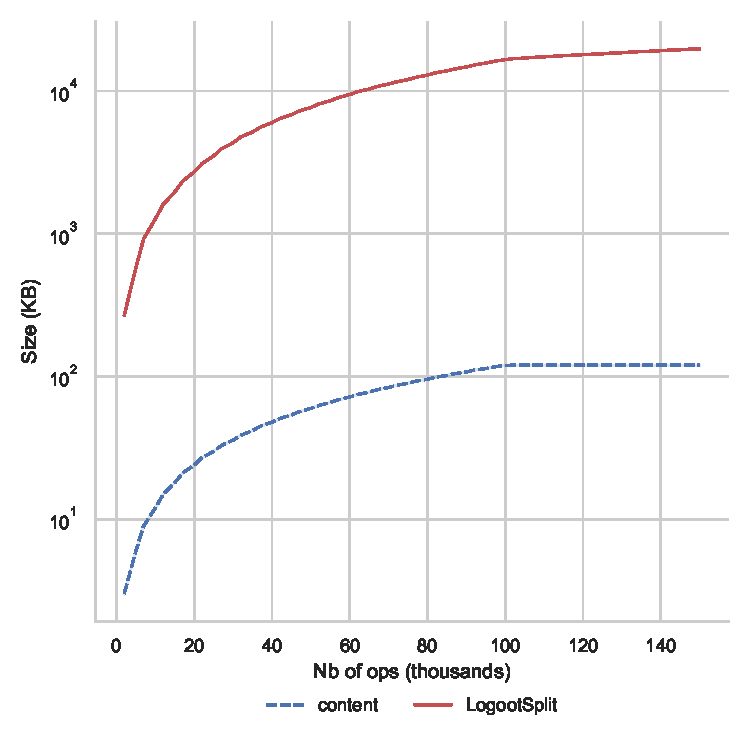
\includegraphics{img/ls-vs-content-snapshot-sizes-7k5.pdf}
  }
  \caption{Taille du contenu comparé à la taille de la séquence LogootSplit}
  \label{fig:size-snapshots-content-vs-ls}
\end{figure}

Sur cette figure, nous représentons l'évolution au fur et à mesure que des modifications sont effectuées sur une séquence LogootSplit de la taille de son contenu, sous la forme d'une ligne pointillée bleu, et de la taille de la séquence LogootSplit complète, sous la forme d'une ligne continue rouge.
Nous constatons que le contenu représente à terme moins de 1\% de taille de la structure de données.
Les 99\% restants correspondent aux métadonnées utilisées par la séquence répliquée, \ie la taille des identifiants, les blocs composant la séquence LogootSplit, mais aussi la structure de données utilisée en interne pour représenter la séquence de manière efficace.

Nous jugeons donc nécessaire de proposer des mécanismes et techniques afin de mitiger les problèmes soulignés précédemments.

\mnnote{
  TODO: Serait plus intéressant de proposer des stats sur la taille des ids, le nombre de blocs composant la séquence, le nombre d'éléments par blocs et la proportion de la taille du contenu sur la taille de la structure de données en fonction du nombre d'opérations jouées.
  Pose la question de quand introduire le protocole suivi pour générer les traces.
}
